% Q5: the solution of 16-x^2 >= 0 and x^2-x-6 > 0.
% Exact endpoints: closed at -4,4; open at -2,3.
\begin{center}
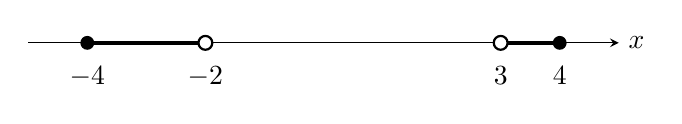
\begin{tikzpicture}[x=0.75cm,y=1cm,>=stealth]
  \draw[->] (-5,0)--(5,0) node[right] {$x$};
  \draw[very thick] (-4,0)--(-2,0) (3,0)--(4,0);
  \fill (-4,0) circle (2.5pt);
  \fill (4,0) circle (2.5pt);
  \draw[fill=white,thick] (-2,0) circle (2.5pt);
  \draw[fill=white,thick] (3,0) circle (2.5pt);
  \node[below=5pt] at (-4,0) {$-4$};
  \node[below=5pt] at (-2,0) {$-2$};
  \node[below=5pt] at (3,0) {$3$};
  \node[below=5pt] at (4,0) {$4$};
\end{tikzpicture}
\end{center}
